\documentclass[12pt]{report}

\usepackage[utf8]{inputenc}
\usepackage{graphicx}
\graphicspath{ {images/} }
\usepackage{float}

\usepackage[a4paper,width=150mm,top=25mm,bottom=25mm]{geometry}

\usepackage{fancyhdr}
\pagestyle{fancy}

% For citations
\usepackage[backend=bibtex]{biblatex}
\addbibresource{Final_Paper.bib}
\usepackage{hyperref}
\hypersetup{
  linkcolor=blue,
  citecolor=blue,
  urlcolor=blue
}

\usepackage{xcolor}
\definecolor{codebgnd}{rgb}{0.9, 0.9, 0.9}
\usepackage{listings}
\lstset{
  basicstyle=\footnotesize\ttfamily,
  breaklines=true,
  backgroundcolor=\color{codebgnd}
}
\hypersetup{colorlinks=true,linkcolor=blue}
% For citations and urls in captions
\usepackage{caption}


\title{
  {Ethernet on the Zynq ZC706 \vspace{0.2in}}\\
  {\large 18-545 Advanced Digital Design \vspace{0.2in}}\\
  {
\includegraphics[width=2in]{cmu_seal.png}}
}

\author{Terence An, Eddie Nolan, Dale Zhang}
\date{December 12, 2015}

\begin{document}
\maketitle

\chapter{Introduction}
This report is a guide to start building ethernet on the Zynq ZC706 board. It was originally written as the final project for a 18-545 project which our team didn't complete because we were unable to build an ethernet adapter in programmable logic and have it properly communicate with the Processing System. The intention of this report is to aid future groups in completing an ethernet adapter, as well as providing the necessary background and deterring groups from fruitless avenues. This guide expects a minimal understanding of Vivado because most students in 18-545 have had limited exposure to it. We will attempt to provide the pertinent references as needed.

That being said, going through Lab 2 in \textit{Vivado Design Suite Tutorial} \cite{vivado_tut} will probably be the fastest way to understand the work flow. Also, chapter 2 and chapter 4 of \textit{UltraFast Design Methodology Guide for the Vivado Design Suite} \cite{ultrafast} will be superbly helpful in learning to use Vivado, especially for using Intellectual Property (IP) in Vivado. Finally, if you still want more details on using IP, you can refer to the Vivado guide on \textit{Designing with IP} \cite{IP} and \textit{Designing IP Subsystems Using IP Integrator} \cite{IP_subsystems}. If you'd like more information on Vivado in general, refer to the \textit{Getting Started} \cite{starter} guide and the \textit{Designs Flows Overview} \cite{design_flows}.

\chapter{Ethernet Background}
In this chapter we'll provide the basics of ethernet, just enough to get you started.
Our discussion will start at the lowest level, and work our way up to the peripheral port on the processing system. If any of these sections are found to be lacking, you can find more information from the 802.3ab standard available on the \href{http://standards.ieee.org/about/get/802/802.3.html}{IEEE Standard Association}. Wikipedia is also your friend.
While the intention of this book is to help you build your own ethernet,
we dissuade people from actually implementing the physical transmission circuitry (PHY) yourself (the PCS and the PMA). The PMA layer is reasonable, but the PCS layer is incredibly involved. If that is all you intend to build for the semester, then perhaps it is possible. Instead we recommend you use the Vivado IP. So we'll simply provide an overview of what these parts do, and if you'd like to build these subsystems yourself, you'll have to refer to the 802.3 documentation.

\section{Logical Link Layer}
The logical link layer may also be referred to as the physical layer.
This network layer deals with how the bits are formatted into frames and how they're transmitted.
If you've worked on any networking projects previously, you could probably just skip this section.

\subsection{Ethernet Frame}
In Figure \ref{fig:eframe} you can see the basic format. However, there is another format for supporting larger frames called jumbo frames, so if frames don't look like what you're expecting that is a possibility. But it isn't very likely, because although most switches and routers support jumbo frames, they're not widely used. While we show the format of the frame, the logical link layer doesn't ascribe any meaning to these bits.

\begin{figure}[!h]
\centering
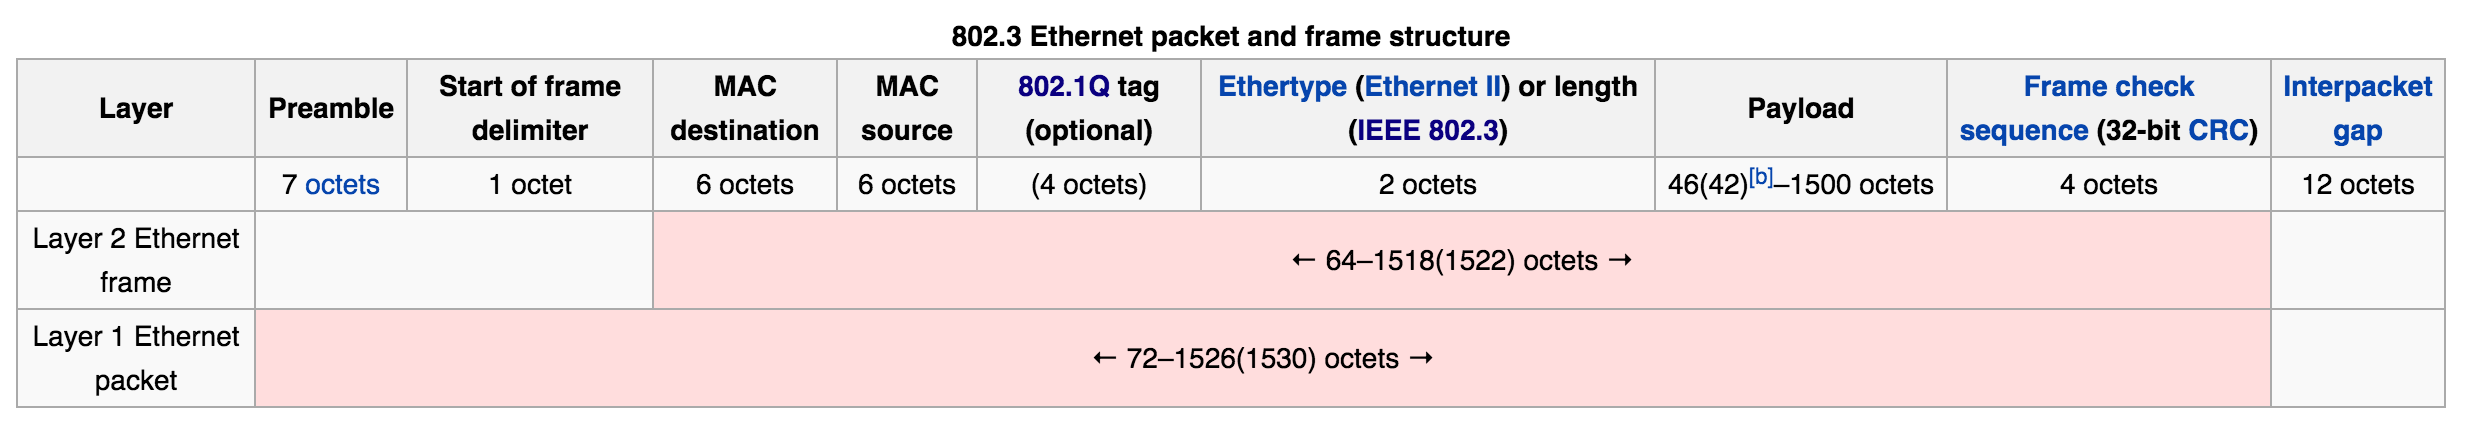
\includegraphics[width=6in]{eframe}
\caption{Ethernet Frame Format}
\small source:\url{https://en.wikipedia.org/wiki/Ethernet_frame}
\label{fig:eframe}
\end{figure}

The layer one bit sequence is what you'd expect to find on the wire, and the layer two format is what you'd expect to reach the operating system.

If there are other headers you're expecting, they'd be in the beginning of the payload. All information used by higher network layers would be found there as well. The standard maximum transmission unit is 1500 bytes, so if you're making a large download, it' be broken up into roughly 1500 byte chunks, each sent according to some higher level protocol like TCP or UDP and your application will receive them in these chunks.

Ethernet frames are sent across Cat-5 or Cat-6 cables, and you'll often see the cables referred to as full-duplex or half-duplex. Duplex refers to the two directions of traffic, tranmissions and receptions. A half-duplex cable/port alternates between transmit mode and receive mode, whereas a full-duplex cable/port has two seperate physical mediums allowing it to transmit and receive at the same time thus removing the need for any collision detection. You'll most likely be using the 1000Base-T standard (802.3ab, the twisted-pair copper standard for 1000Mbs as opposed to 1000Base-X, the fiber optic standard for 1000Mbs) which only operates on full-duplex.

The frame is transmitted 8 bits at a time over these wires, but they're encoded,
so if you wanted to parse these bits yourself it's a little bit more complicated.
We'll discuss more about this in the PMA section.

\subsection{Physical Medium Attachment (PMA)}
The PMA is the first subsystem that connects to the actual wires which is called the Medium Dependent Interface (MDI). The signals then are transmitted to a PCS PMA interface.
The PMA is fairly straight forward to implement, you simply have to properly implement a very brief transmit function, receive function, reset function, link monitor function, clock recovery function, and a fairly lengthly control function. The exact details can be found in the 802.3z standard, section 40.4.3. Figure \ref{fig:pma} gives a succinct overview of how the signals are used and generated.


The MDI consists of 4 wires for each transmission direction and each wire can take of 5
different voltages which we'll label as \{2,1,0,-1,-2\}.
The transmit side constantly changes the voltage, even when idle.
During idle, the voltages oscillate from 2 to 0 to -2 and back.
The baud rate is 125 MBaud which matches the clock rate of 125 MHz so there's one symbol per 8 ns.

\begin{figure}[H]
\centering
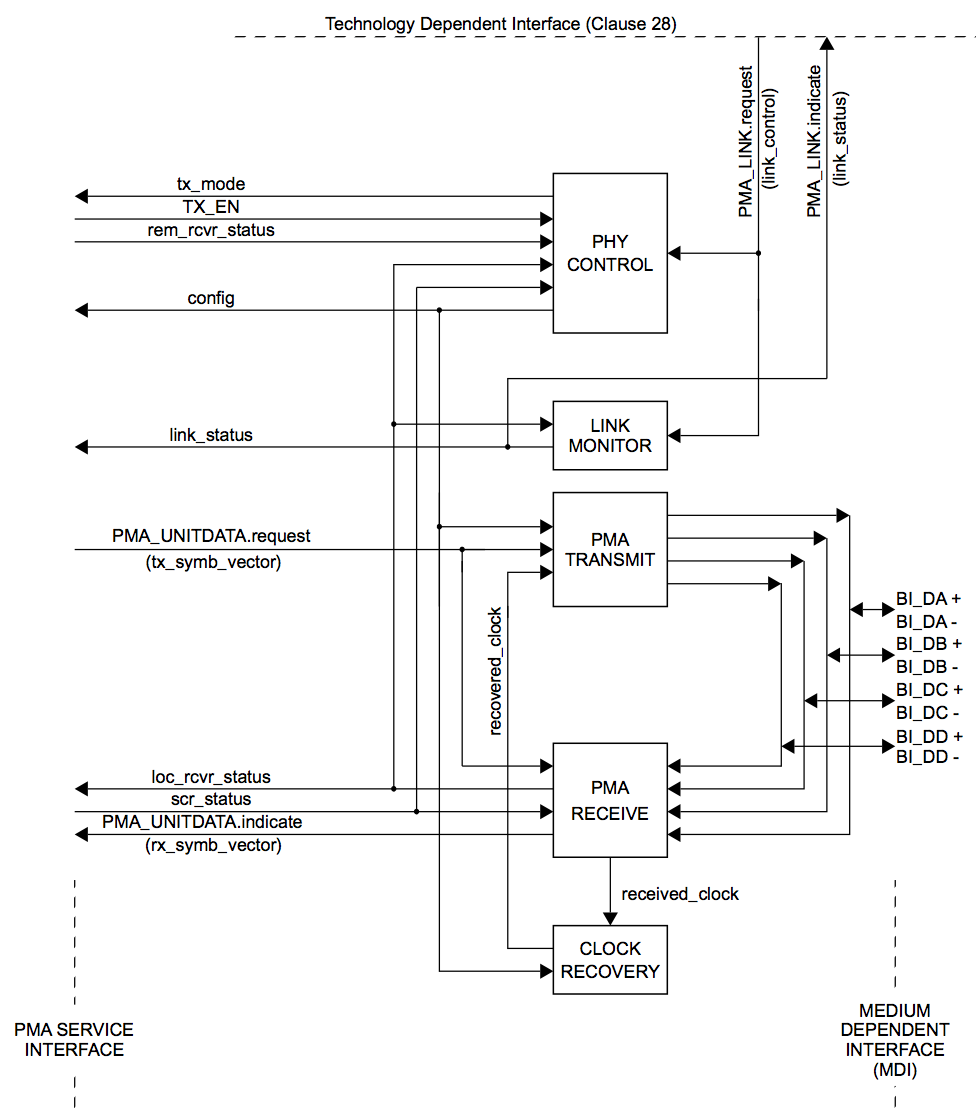
\includegraphics[width=4in]{pma}
\caption{PMA Reference Diagram}
\small source:802.3z Standard 40.4.3, Figure 40-13 \cite{802.3z}
\label{fig:pma}
\end{figure}

\subsection{Physical Coding Sublayer (PCS)}
The PCS is the subsystem that connects from the PMA to the Media Independent Interface (MII).
Because this guide is for 1000Base-T, our PCS must interface to Gigabit Media Independent Interface (GMII) or the Reduced GMII (RGMII).
In figure \ref{fig:pcs} you can see an overview of the PCS function. However, it hides a lot
of complexity. Implementing your own PCS is a very large undertaking,
despite the small reference diagram. It might appear as if you only have to implement
the transmit function, the transmit enable, collision detection, and the receive function.
The transmit function alone, is monumental.
We have to convert the bit stream into 4 wire code groups,
where each byte is encoded using the 4D-PAM5 technique into 4 quinary symbols.
We also have to scramble these symbols with a linear feedback shift technique.
The exact specifications can be found in section 40.3.1.3 in the 802.3z standard.
The state diagram can be seen in figure \ref{fig:pcs_transmit}.

\begin{figure}[H]
\centering
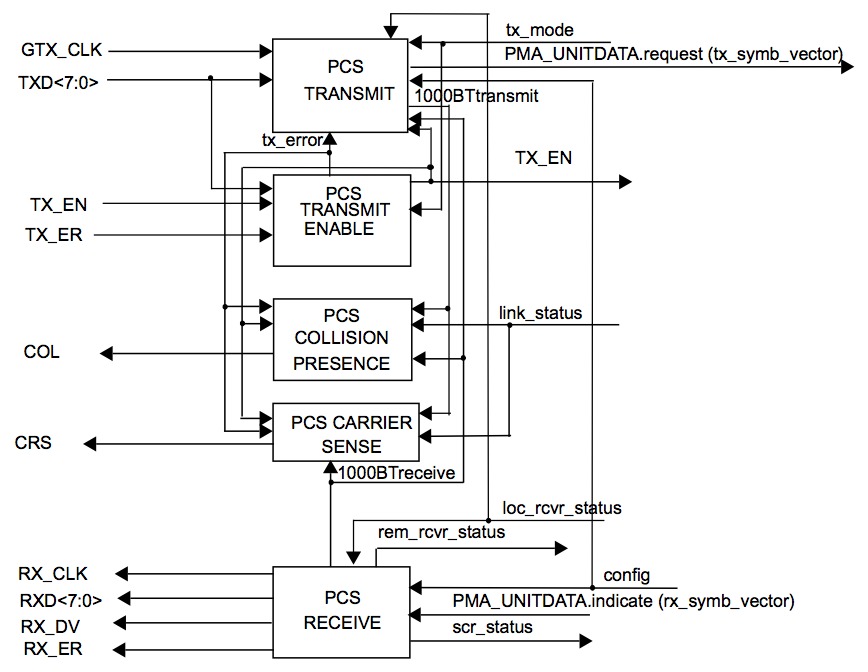
\includegraphics[width=4in]{pcs}
\caption{PCS Reference Diagram}
\small source:802.3z Standard 40.3.1, Figure 40-5 \cite{802.3z}
\label{fig:pcs}
\end{figure}

\begin{figure}[H]
\centering
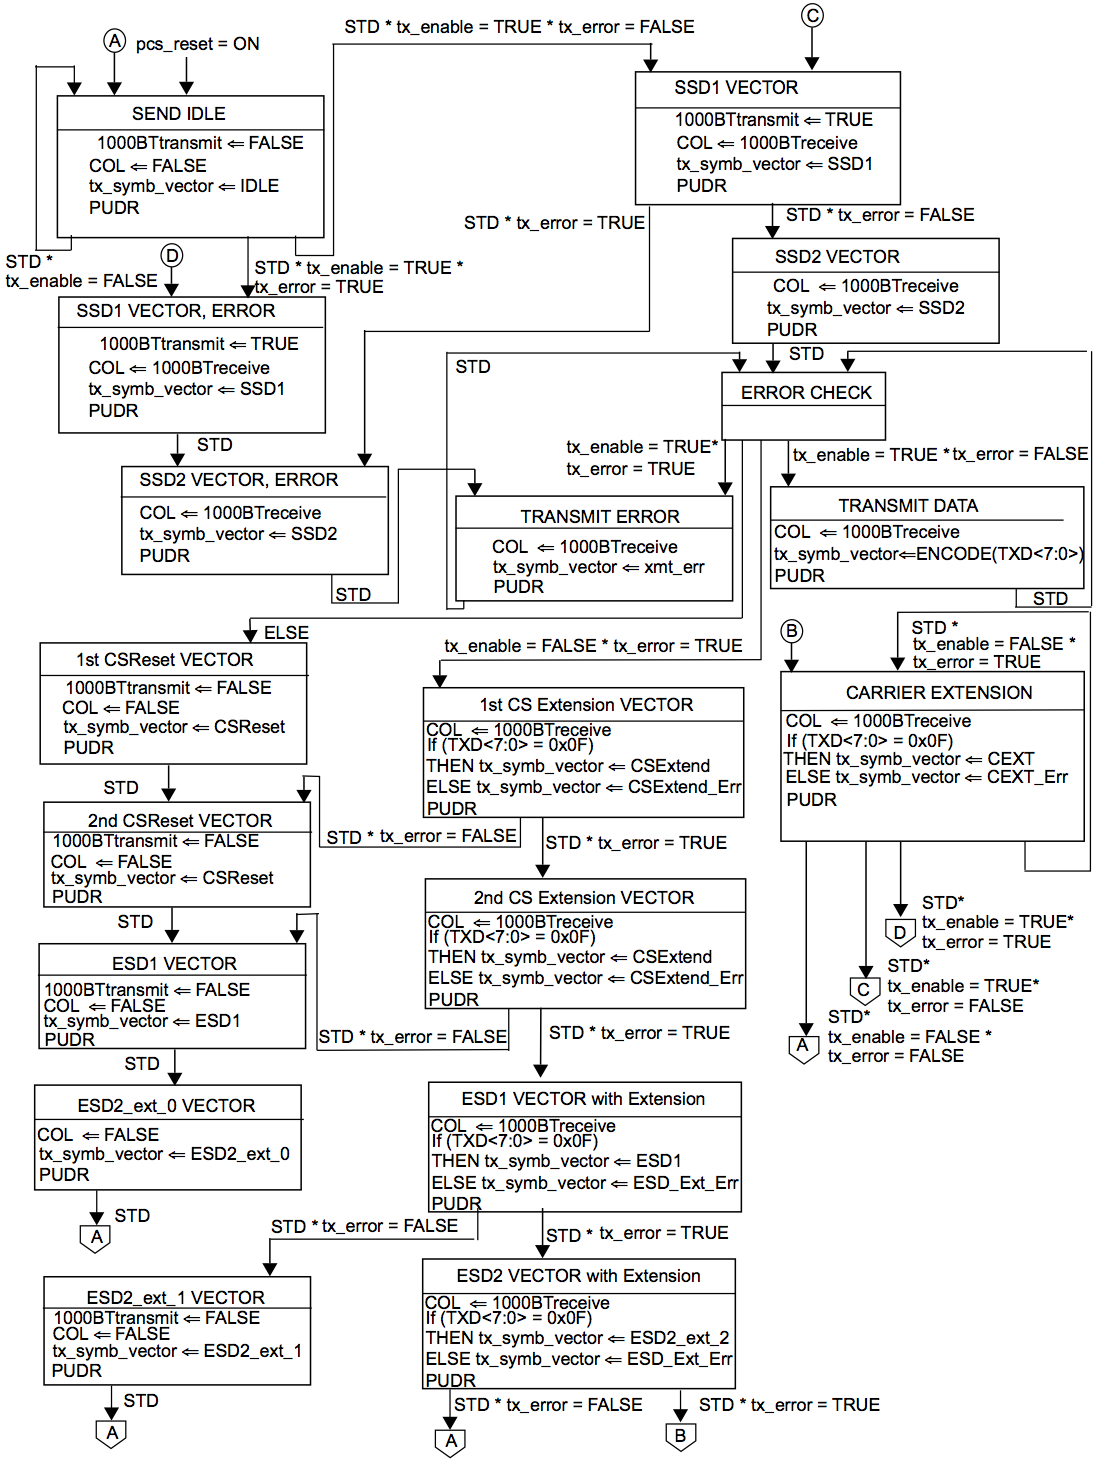
\includegraphics[width=4in]{pcs_transmit}
\caption{PCS Transmit State Diagram}
\small source:{802.3z Standard 40.3.4, Figure 40-9} \cite{802.3z}
\label{fig:pcs_transmit}
\end{figure}

Luckily though, the PCS for 1000Base-T doesn't haven't to handle collision detection since
1000Base-T is full duplex.
The PCS also uses the MII's managment interface to handle Auto-Negotiation which is required
in 1000Base-T.

\section{Data Link Layer}
The data link layer is comprised of two sublayers,
but this would be the format an operating system sees.
The layer one ethernet frame has its preamble and start of frame delimiter dropped by the MAC subsystem. Remember that the logical link layer was agnostic to the ethernet frame format.
It is only the MAC that understands which bits are which part.
\subsection{Logical Link Control}
This sublayer is higher up than the MAC and handles network control frames. It handles higher level network protocols like IP, Decnet, Appletalk, etc. We can ignore these for your ethernet subsystem.
Technically, a part flow control also resides in this sublayer,
but for LAN protocols like ethernet there is no flow control in this sublayer.
\subsection{Media Access Control (MAC)}
This sublayer interprets the bit stream into a MAC ethernet frame, checks for frame errors, and passes on the frame in its disessembled form in reception mode. When transmitting, it takes the frame, adds the preamble and start of frame delimiter and adds its own source MAC address. It is important to know that the order of transmission is by one octel at a time with the low-order bits first. Usually the MAC handles collision detection as well, and carrier sense, but since we have full-duplex you can ignore these. In short, the MAC interprets the signals from the GMII and sends the layer 2 ethernet frame to the processing system.

\chapter{Basic Approach}
I will assume that your project is not to just implement the PHY and you're trying to build something on top of the PHY because if all you wanted to do was build the PHY yourself, the background chapter is all you need. This chapter is about how to quickly get started on making ethernet in programmable logic, and how you might modify it to make additions to it.

After numerous failed attempts, we finally settled on using the Zynq PL Ethernet \cite{zynq_pl_eth} guide on the Xilinx Wiki; however, we never got it completely working before the semester ended. Had we discovered it earlier, and decided on going down this route earlier, perhaps things would have been different. Also, when we actually started using it, it was in flux. Someone was editting the page still, writing the 2015 version (XAPP1082 v4.0); so we ended up using the 2014 version (XAPP1082 v3.0). But by the time you've seen this guide, there will definitely be a 2015 version and possibly even newer ones.

Perhaps you can follow the wiki guide right now, and all the steps work for you right off the bat.
For us, it didn't turn out this way.
The guide in general is great, and it went smoothly for most of the way until we ran into a problem with the PetaLinux network stack.
We'll discuss PetaLinux more in depth in a later chapter because that discussion will be sizeable in and of itself. So for the rest of this chapter, I'll be mostly explaining what the steps in the wiki are doing so that you will be able to modify their setup. There's no need to cover each instruction, I'll just comment on the ones that warrant an explanation for a beginner. Remember, the instructions I'll be covering are for version 3, so you'll have to translate it yourself for later versions.

\section{Building PL Ethernet}
First of all, we're not interested in the PS-EMIO design on the wiki since that uses the built in Marvel chip as the ethernet adapter and it connects to the processing system through the Extended Multiuse I/O (EMIO). There is very little we can modify in that design. Rather, scroll down until you find the section titled \textbf{Building PL Ethernet}. It will tell you to run a tcl script which is how vivado allows you to script building designs. At the top you'll see it specify a vivado version number as well as the board number this script was made for. The script you download from this wiki will be for the ZC706 board. Following the next few steps will get you a bitstream, but know that this process can sometimes take up to an hour. So make sure you export it to the SDK. When you export, if you leave the path as ``$<$ local to project $>$`` you'll only be able to save one bitstream, so if you wanted a backup you'd need to make a seperate directory for it.

That was it as far as the programmable logic goes!
Of course you should understand the design and what each block is doing in order to modify it.
I'll go more into detail about each IP later, but the overall receive pipeline is that the SFP
port connects to the PCS/PMA IP then to the TEMAC through the Serial GMII (SGMII) interface.
The Tristate-Ethernet MAC (TEMAC) connects to the DMA block through an AXI-stream interface
which then connects to the Processing System through the high performance AXI ports.
In the transmission direction it's the same pipeline but backwards except instead of the HP port,
the processing system connects to the General Purpose interconnect which then connects to the DMA.
So if you wanted to analyze, filter, or modify the packets at the layer 2 level you should
insert your own RTL after the TEMAC.

\section{The PHY IP}
The Vivado IP catalog thankfully has all the parts of the PHY you'll need. You'll have to be comfortable with using and making your own IP to work well in Vivado. Xilinx already has implementations of the PCS, PMA, MAC, etc. and they're in blocks which they call their Intellectual Property (IP). You can find the documentation on all of these on their website (there is a button to open them directly in vivado, but that button doesn't do anything. Get used to this). Their IP blocks communicate via a protocol called AXI4. You'll want to skim through The Zynq Book \cite{the_zynq_book} to understand AXI well. In general The Zynq Book doesn't go enough into detail, but for AXI it is still alright.

\section{Modifying the pipeline}
This setup they provide will move the whole data frame into memory. So the easiest place to add your own modifications is to the AXI-stream connect after the TEMAC and before the DMA. The modification we worked on was adding a filter to the output AXI of the TEMAC. Vivado\_HLS is a high level synthesis tool that allows you to write C and C++, and it'll be compiled down to an HDL which is packaged inside of an IP. This IP will be added to your IP catalog so you can select it inside of Vivado. The function arguments are your input and output ports. You can set the ports to have difference interfaces using PRAGMAs, but @TODO

If you want one of your ports to connect to the processing system, leave it unconnected in the block diagram, and add it to the address editor. Vivado will set up the connections automatically.

\chapter{PetaLinux Networking}
\subsection{Introduction}
This section will focus on the attempts we made to implement the software-firmware stack that Xilinx provides through their application notice XAPP1082 and through a guide on the Xilinx wiki. This involves creating a bootable SD card containing a copy of PetaLinux, Xilinx's embedded Linux distribution, that is patched to support communicating over the SFP Ethernet port, and flashing the FPGA fabric with a corresponding bitstream that implements the hardware Ethernet support. Although our eventual goal was to modify the kernel and firmware to support Ethernet traffic analysis, we ran into bugs that we were unable to fully diagnose and solve.
\subsection{Relevant Hyperlinks and Documentation}
\begin{itemize}
  \item \href{http://www.xilinx.com/support/documentation/application_notes/xapp1082-zynq-eth.pdf}{XAPP1082 PDF}
  \item Xilinx Wiki Guides:
    \begin{itemize}
    \item \href{http://www.wiki.xilinx.com/Zynq+PL+Ethernet}{Zynq Ethernet Guide}
    \item \href{http://www.wiki.xilinx.com/Prepare+Boot+Medium}{Zynq Boot Setup Guide}
    \end{itemize}
  \item \href{http://www.xilinx.com/support/documentation/boards_and_kits/zc706/ug954-zc706-eval-board-xc7z045-ap-soc.pdf}{Zynq ZC706 User Guide}
  \item \href{http://www.xilinx.com/support/documentation/sw_manuals/petalinux2014_4/ug1144-petalinux-tools-reference-guide.pdf}{PetaLinux Tools Reference Guide}
  \item \href{http://www.silabs.com/products/mcu/Pages/USBtoUARTBridgeVCPDrivers.aspx}{Drivers for Zynq ZC706 UART}
\end{itemize}
\subsection{Supplies}
\begin{itemize}
  \item Hardware: 
    \begin{itemize}
    \item It's necessary to be able to connect to a wired Ethernet connection and write SD cards with the computer you are using for development.
    \item If you want to switch between different copies of PetaLinux, it's convenient to have multiple SD cards, so you don't have to reflash them repeatedly. The copy of PetaLinux we used was only ~200MB so large storage capacity is unneccessary.
    \item It's helpful to have an Ethernet switch or router so you can test the device without needing access to the full Internet.
    \end{itemize}
  \item Software:
    \begin{itemize}
    \item I installed the PetaLinux tools on two Ubuntu LTS virtual machines. You should have virtualization software and enough disk space available on your computer for 2 virtual machines.
    \item We also were able to use lab computers that were configured to use the version of Vivado that corresponded to the version of XAPP1082 we used.
    \item The specific versions that our project used were XAPP1082 version 3, PetaLinux and Vivado version 2014.4, Xubuntu 14.04 LTS for installing the PetaLinux tools. Our lab machines ran RHEL.
    \end{itemize}
\end{itemize}

\section{Using PetaLinux}
\subsection{Creating Boot Media}
The Zynq Boot Setup Guide linked above demonstrates the way to format bootable SD cards. You need to create 2 partitions, \texttt{boot} and \texttt{root}, and copy 2 files, \texttt{BOOT.bin} and \texttt{image.ub}, onto the 'boot' partition, but the partition table needs to be configured in a specific way using fdisk commands. The relevant part of the guide is the section under ``SD Boot''; ignore the sections that describe JTAG and QSPI booting. You can find relevant precompiled \texttt{BOOT.bin} and \texttt{image.ub} files in the XAPP1082 software release: \texttt{\$XAPP\_HOME/ready\_to\_test/pl\_eth\_noCso}.

\subsection{Building XAPP1082's PetaLinux Configuration}
The version of the PetaLinux Tools that we used wouldn't install properly on a 64-bit virtual machine because of issues with 32-bit library support that we were unable to resolve. However, the Xilinx SDK, which is required to create the boot image after the kernel has been compiled, only supports 64-bit versions of Linux. We were able to get around this by creating a 32-bit VM for creating the project and building the kernel, and a separate 64-bit VM for creating the boot image.

\subsubsection{Setting up the 32-bit VM}
For Ubuntu, the PetaLinux Tools Reference Guide required the following packages to be installed:
\newline \texttt{tofrodos iproute gawk gcc git-core make net-tools libncurses5-dev tftpd zlib1g-dev flex bison}

The PetaLinux Tools are distributed as a self-extracting archive/installer. The Xilinx Wiki Zynq Ethernet Guide contains a download link. Both the PetaLinux Tools and the XAPP1082 software release should be extracted. The provided shell scripts help to automate steps that are described in the Wiki guide. The directories on the first lines should be modified to reflect the user's configuration.


\subsubsection{Setting up the 64-bit VM}
To set up the 64-bit VM, you need to install all the same packages as the 32 bit VM needs. In addition to extracting the PetaLinux installer, you also need to install the Xilinx SDK that corresponds to your version of PetaLinux. After you have finished configuring and building the project on the 32-bit VM, you can copy the \texttt{xapp1082\_pl\_eth} project directory to the 64-bit VM, then use the provided shell script to create a bootable image (more detail is available in the wiki guide). The required files for creating a bootable SD card will be in the project directory in the subdirectory \texttt{images/linux}.

\subsubsection{Note on PetaLinux Setup}
In an attempt to diagnose the main problem that we encountered, we needed to introduce a change to the Xilinx ethernet driver so that it would print debug information. We did this by text-editing the patch file that adds driver support to the kernel, although there are many other ways of modifying the PetaLinux configuration and software that are described in more detail in the documentation. If there is no need to customize PetaLinux in any way, precompiled images are provided in the XAPP1082 software release, and the PetaLinux Tools don't need to be used.

\subsection{Connecting to the UART of the Zynq ZC706}
The driver download page for the ZC706 can be found in the link section. After the drivers are installed, remote terminal software can be used to communicate with the ZC706. We found it easiest to use \texttt{screen}. If the UART shows up as \texttt{/dev/ttyUSB0}, the ZC706 can be connected to by running \texttt{screen /dev/ttyUSB0 115200}. Permissions issues can often prevent reading from device files so it's important to ensure that permissions are set properly.

\subsection{PetaLinux Networking Setup}
\subsubsection{SFP Ethernet Port}
As described in the Xilinx Wiki guide, to activate the interface for the SFP Ethernet port, you should run
\newline \texttt{insmod /lib/modules/3.17.0-xilinx-<kernel\_build\_version>/kernel/}
\newline \texttt{drivers/net/ethernet/xilinx/xilinx\_axienet\_main.ko}
\newline This loads the kernel module that enables the SFP Ethernet interface.
\newline To activate the interface, run
\newline \texttt{ifconfig eth1 up x.x.x.x}
\newline where \texttt{x.x.x.x} is the IP address assigned to the SFP interface.
\newline You should see the following two messages:
\newline \texttt{eth1: XAXIEthernet: PHY Link carrier lost.}
\newline \texttt{eth1: XAXIEthernet: PHY Link carrier restored.}
\newline If the second message does not appear, that means that Petalinux is unable to set the link up. This is the problem that our team encountered that we were unable to move past.

\subsubsection{Configuration}
Unfortunately, the tools that are included by default in the provided PetaLinux configuration are limited; in particular, there is no DHCP support. In order to set up an interface, you will need to know you're device's:
\begin{itemize}
\item Assigned IP address
\item Broadcast address
\item Network mask
\item Default gateway
\end{itemize}
The default gateway can be set by running:
\newline \texttt{route add default gateway x.x.x.x}
\newline You can set the IP address and activate the interface by running:
\newline \texttt{ifconfig eth0 up x.x.x.x}
\newline Use ifconfig to add the netmask and broadcast address:
\newline \texttt{ifconfig eth0 broadcast x.x.x.x}
\newline \texttt{ifconfig eth0 netmask x.x.x.x}
\newline If your configuration works, you should be able to connect to the internet. 

\subsection{Bugs and Roadblocks}
The bug that we were unable to overcome in our project was that Petalinux was unable to successfully set the link up for the SFP port interface. The Xilinx Wiki advised us to make sure we saw the message
\newline \texttt{eth1: XAxiEthernet: PHY Link carrier restored.}
\newline before using the SFP interface. We never encountered this message. Here is the part of the driver code that triggers this message:
\begin{lstlisting}[language=C]
if (phy_carrier) {
  printk(KERN_INFO
         "%s: XAxiEthernet: PHY Link carrier restored.\n",
         dev->name);
  netif_carrier_on(dev);
  set_mac_speed(lp);
}
\end{lstlisting}
The variable \texttt{phy\_carrier} is set to the value of \texttt{linkup} in the \texttt{get\_phy\_status} function:
\begin{lstlisting}[language=C]
static int get_phy_status(struct net_device *dev, DUPLEX * duplex, int *linkup)
{
	struct axienet_local *lp = (struct axienet_local *) netdev_priv(dev);
	u32 reg1, reg2;

	//reg1 = axienet_mdio_read_local(lp, lp->gmii_addr, MII_BMCR);
	reg1 = axienet_mdio_read(lp->mii_bus, lp->gmii_addr, MII_BMCR);
	*duplex = FULL_DUPLEX;

	//reg2 = axienet_mdio_read_local(lp, lp->gmii_addr, MII_BMSR);
	reg2 = axienet_mdio_read(lp->mii_bus, lp->gmii_addr, MII_BMSR);
	*linkup = (reg2 & BMSR_LSTATUS) != 0;

	//printk(KERN_ERR "get_phy_status: BMCR=0x%x, BMSR=0x%x, duplex=%d, linkup=%d\n", reg1, reg2, *duplex, *linkup);
	return 0;
}
\end{lstlisting}
Reading the driver code showed that the status and control values that the SFP device was providing to the MII interface didn't indicate that the Ethernet link was up. We modified the driver code to uncomment the call to \texttt{printk}, which showed us that the MII control register value was always 0x1140, while the status register was always 0x01c8. The values are bitmasks that we interpreted the following way:
\begin{verbatim}
MII Basic Mode Status Register
Bit 0: Extended MII registers available
Bit 1: Jabber detected (sticky)
Bit 2: Link is up (sticky)
Bit 3: Capable of auto-negotiation
Bit 4: Remote fault detected
Bit 5: Auto-negotiation complete
Bits 6-A: unused
Bit B: Capable of 10mbps half-duplex
Bit C: Capable of 10mbps full-duplex
Bit D: Capable of 100mbps half-duplex
Bit E: Capable of 100mbps full-duplex
Bit F: Capable of 100mbps 4k packets

Value we get from ZC706: 0x01c8

 F E D C B A 9 8 7 6 5 4 3 2 1 0
|0|0|0|0|0|0|0|1|1|1|0|0|1|0|0|0|

MII Basic Mode Control Register
Bits 0-6: unused
Bit 7: Collision test
Bit 8: Full duplex
Bit 9: Autonegotiation restart
Bit A: Disconnect PHY from MII
Bit B: Power down PHY
Bit C: Enable autonegotiation
Bit D: Select 100mbps
Bit E: TXD loopback bits
Bit F: Reset

Value we get from ZC706: 0x1140

 F E D C B A 9 8 7 6 5 4 3 2 1 0
|0|0|0|1|0|0|0|1|0|1|0|0|0|0|0|0|
\end{verbatim}

Some of these reported settings and status bits make sense, but some do not; no status bit is set that says that the PHY is able of any particular Ethernet link speed, but at the same time both the status and control registers say that the device is configured for autonegotiation.

This was as far as we were able to get with debugging this issue. Something we would have wanted to test was whether the SFP port acted differently with a different module. The XAPP1082 PDF specified that it was tested with a ``HP 378928-B21 Cisco Gigabit Ethernet RJ45 SFP Module,'' whereas our SFP module was a different brand and model.

\subsection{Other Notes}
\begin{itemize}
\item Make sure jumper J17 is set (see XAPP1082 PDF)
\end{itemize}
\subsection{Code Listing}
\subsubsection{Shell Scripts for the 32-bit VM}
\texttt{1\_create\_project\_config\_kernel.sh}
\lstinputlisting{shellscripts/1_create_project_config_kernel.sh}

\texttt{2\_apply\_patch\_build\_kernel.sh}
\lstinputlisting{shellscripts/2_apply_patch_build_kernel.sh}

\subsubsection{Shell Script for the 64-bit VM}
\texttt{3\_create\_boot\_image.sh}
\lstinputlisting{shellscripts/3_create_Boot_image.sh}

\chapter{Alternate Approaches}
The first approach we attempted was to build our own ethernet system. From the background chapter, I hope I've gotten across the difficulty of doing so. I thought I could just watch the line for a preamble, and start reading the bits after a start of frame delimiter. The more I read and researched the more layers of complexity I realized existed ontop of such a seemlingly simple operation. Then apart from just reading bits, transmitting and the other protocols and interfaces to conform to made this infeasible.

So we then looked more into a paper \cite{pp} I found describing a high level language Xilinx created to compile down into an HDL. This looked promising, but after a few email correspondences with Gordon Brebner, one of the authors of the paper, we learned that the packet processing language (PP) was discontinued by Xilinx. It was split into two, and the lower level portions became SDNet, a proprietary development environment made for building networking technologies. Unfortunately a license for it is very expensive, and it'd also mean we'd have to learn another tool besides Vivado.
The higher level half turned into an open source project called the P4 language.
This compiles a high level language into a number of target languages. Although Gordon was very enthuastic and helpful when it came to this, the P4 language is still very early in it's infancy and we knew there was going to be very little support. The other problem was that targetting Verilog wasn't complete yet, and we'd have to target SDNet anyways. Perhaps in the future, this would be more viable.

I then tried to use their IP myself, and I tried to figure out a viable block design from their documentation. You can find my block diagram in Figure \ref{fig:my_design}.
As far as I can tell, the clocking, the resets, and the axi connections are correct.
The processing system is connected on the correct EMIO ports and memory mapped IO are all set in the address editor, and while this design was verified, it could not synthesize.
And if you look closely at the console in the figure \ref{fig:my_design} you can see one of the most useless error messages I have ever come across.
If it's hard to see, it says \texttt{HDL Generation failed for the IP integrator design /afs/ece.cmu.edu/usr/terencea/Public/18545/.../design\_1.bd}.
It is tautologically true! I didn't need Vivado to tell me this! How do I go about debugging this?
At this point, I couldn't find anymore information on the forums.
Removing pieces just added more external peripheral ports so while some may have synthesized,
they weren't ever useful.

\begin{figure}[H]
\centering
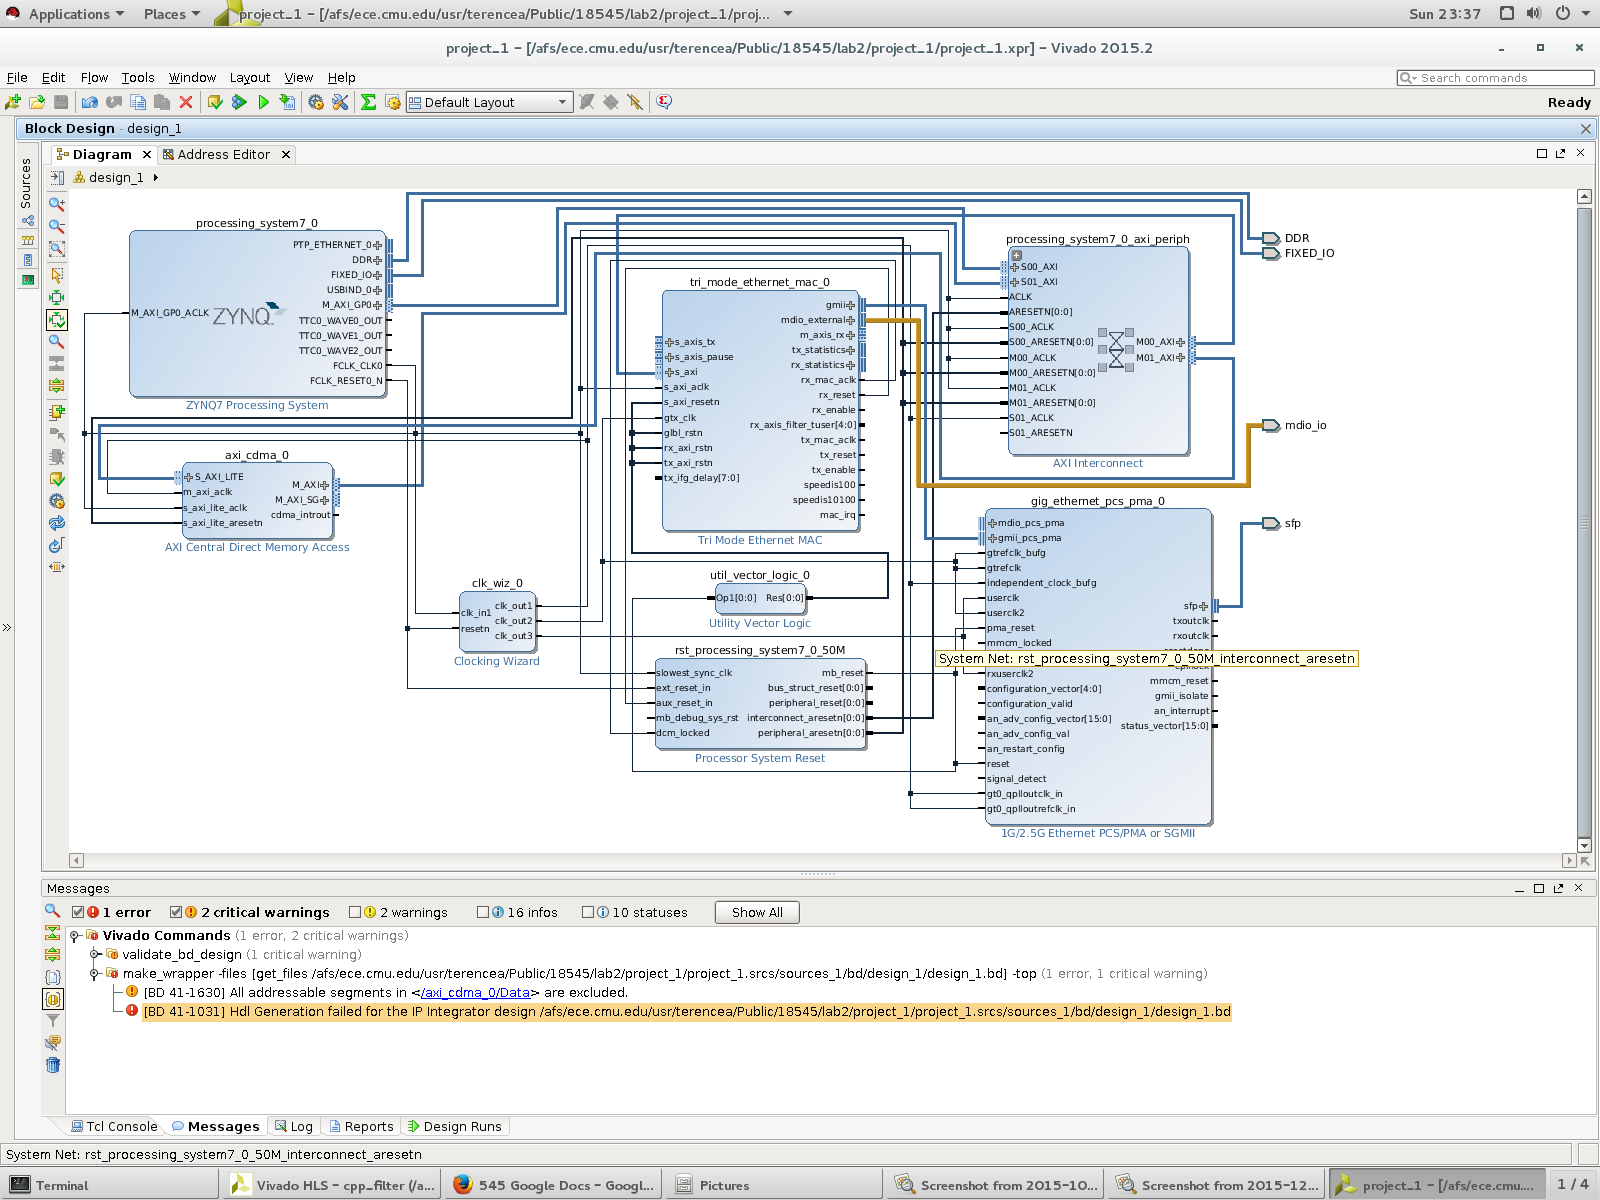
\includegraphics[width=6in]{my_design}
\caption{My PL Block Diagram}
\label{fig:my_design}
\end{figure}

Another wiki guide we tried to follow was \textit{Zynq-7000 AP SoC - Performance - Ethernet Packet Inspection - Linux - Redirecting Packets to PL and Cache Tech Tip} \cite{redirect}. This one looked promising because we could have redirected traffic into PL and done all of our network analysis in hardware. However, it seems to be missing a lot of parts, and there were more edits to this wiki after we first discovered it. So perhaps in the future this wiki will be more useful. But at the time, some file headers were for the Kintex, some for Zynq, and some for Virtex. So it looked like an incomplete tech tip.

\chapter{Lessons Learned}
\begin{itemize}
\item We spent far too much time early in the project doing research. This meant that by the time we felt we had enough knowledge to begin actually working, it was already fairly late in the semester and time was running short.
\item We did not anticipate all the bugs and roadblocks we ran into, some of which could have been tackled earlier in the semester, i.e. registering our device on the school's ethernet to start debugging that earlier.
\item We fell victim to some poorly documented/incorrect guides that we spent large amounts of time trying to force to work. This made it even more discouraging when we did end up abandoning those methods, since we had spent so much time only to have to try to start from scratch again.
\item Relating to the last item, we also depended on following online guides and wikis very heavily, and often blindly, without full understanding of why the guide was supposed to work (or often times, not work).
\item Since our knowledge on getting ethernet onto an FPGA was very limited fromt the start, it was difficult to come up with concrete tasks and distribute them among team members. We should have probably come up with more well-defined tasks, and not just telling team members to "Just get something to work" by a certain date.
\end{itemize}


\chapter{Miscellaneous}
\section{Personal Statements}
\subsection{Terence An}
There is a lot to learn, and a lot that could go wrong. \\
Looking back, the first thing I did wrong was have high expectations. Really. \\
Building this is challenging, and not in the way you'd expect. In reality, there is a correct way to build ethernet in PL and have it properly communicate with Linux, and I suspect that proper solution is probably really short, but really elusive.

The challenge is learning to use Vivado, and trying to find documentation on what you're using. There is no guide that gives you just enough working knowledge to start building anything. It's a lot of trial and error, and Vivado error messages are often horrifically useless.
Almost every piece of documentation you find will be technically correct, full of detailed information, and still somehow utterly useless.
Their IP documentation will tell you the exact timings of every signal, where every piece of I/O is, and at the end of it, you'll still have no clue how to use this particular IP. Instead, looking for example designs and design feedback on the wiki and the forums will be much more helpful. But whatever you do read, know that it often won't be correct. You'll have to fish out the parts you can use, and ignore the rest. A lot of wiki example designs just don't work at all. In the end, get used to starting quickly and restarting often. If this is what you'd like to build, do it! You'll learn a lot, and hopefully you can pick up where we left off. Good luck!

\subsection{Edward Nolan}
One of the challenges that we faced this semester was figuring out how to approach a new topic, networking, that none of us were experts on, without having a blueprint from previous projects to base our experience on.

I think that in addition to the technical experience I've gained from this project, I will also value the lessons I've gained about what works and what doesn't when you're attempting something that you're unfamiliar with. One of the things that our team was good at getting done was doing research and gathering background information. However, there wasn't enough of a sense of urgency to try to act on what we found out, and we should have been ready to ``fail faster'' by testing out different options to see if they were viable as soon as we could.

Another factor that made our project difficult was dealing with inaccurate, incomplete, or outdated documentation. The problem that we were unable to overcome was not mentioned in the Xilinx Wiki guide. Information that came from forums or unofficial sources was more difficult to understand and act on, despite being necessary to move forward with the project. 

We should also have reached out earlier on for help from people with more experience with these topics. The Xilinx forums could have been helpful if we had used them more to ask directly relevant questions, instead of only referencing threads that were started by other engineers. More reliance on outside expertise could also have helped us recognize when our project was on the wrong track.

Overall, although our team didn't achieve what we planned, I enjoyed the experience, and learned a lot about both networking technology and scheduling and working in a group project. Good luck to any future 545 Ethernet teams!

\subsection{Dale Zhang}
For me, this class was challenging for a multitude of reasons. First off, I hadn't touched Verilog since I took 18-240 a few years ago, and I also wasn't very comfortable with HDL. In addition, in the context of our project, I had very little knowledge on ethernet and networking, so I had to learn a lot about how our project worked as I went along.

Over the course of the semester, there are definitely a few things I wish I had done differently. Since Terence and Eddie were both far more knowledgeable about Ethernet and networking, I often took a backseat to them when the group was making decisions. However, at some points in the semester, instead of asking for their help understanding some of the concepts driving our design, I would try to do it myself, without very much success. This led to me spending far more time on some tasks than I should've. This definitely limited my effectiveness as a team member.

Another mistake we made as a team was underestimating how much work actually needed to go into this project. Towards the beginning of the semester, we didn't put in much lab time outside of class periods and mandatory lab time. It first really caught up to us around mid semester with the first status meeting, where we saw how far behind we were, and how much more time we would need to commit for the rest of the semester.

Some advice I'd have for anyone planning to pursue an FPGA Ethernet project in the future is not to spend too much time trying to do research, and to start actually working on the board as soon as possible. In addition, ethernet on FPGA is not very well documented, and much of the documentation available is incorrect or incomplete.

For the class in general, it's definitely better to spend the long hours working on your project earlier in the semester, before your other classes have started to pick up. In addition, at the beginning of the semester, try and pick a project that you can be passionate about and that you would really like to see succeed. At times, I felt very unmotivated to go in an work on the project simply because I wasn't particularly excited about our final product.

To all future students reading this, good luck with the class and have fun!

\printbibliography

\end{document}
